\begin{titlepage}
    \begin{center}
        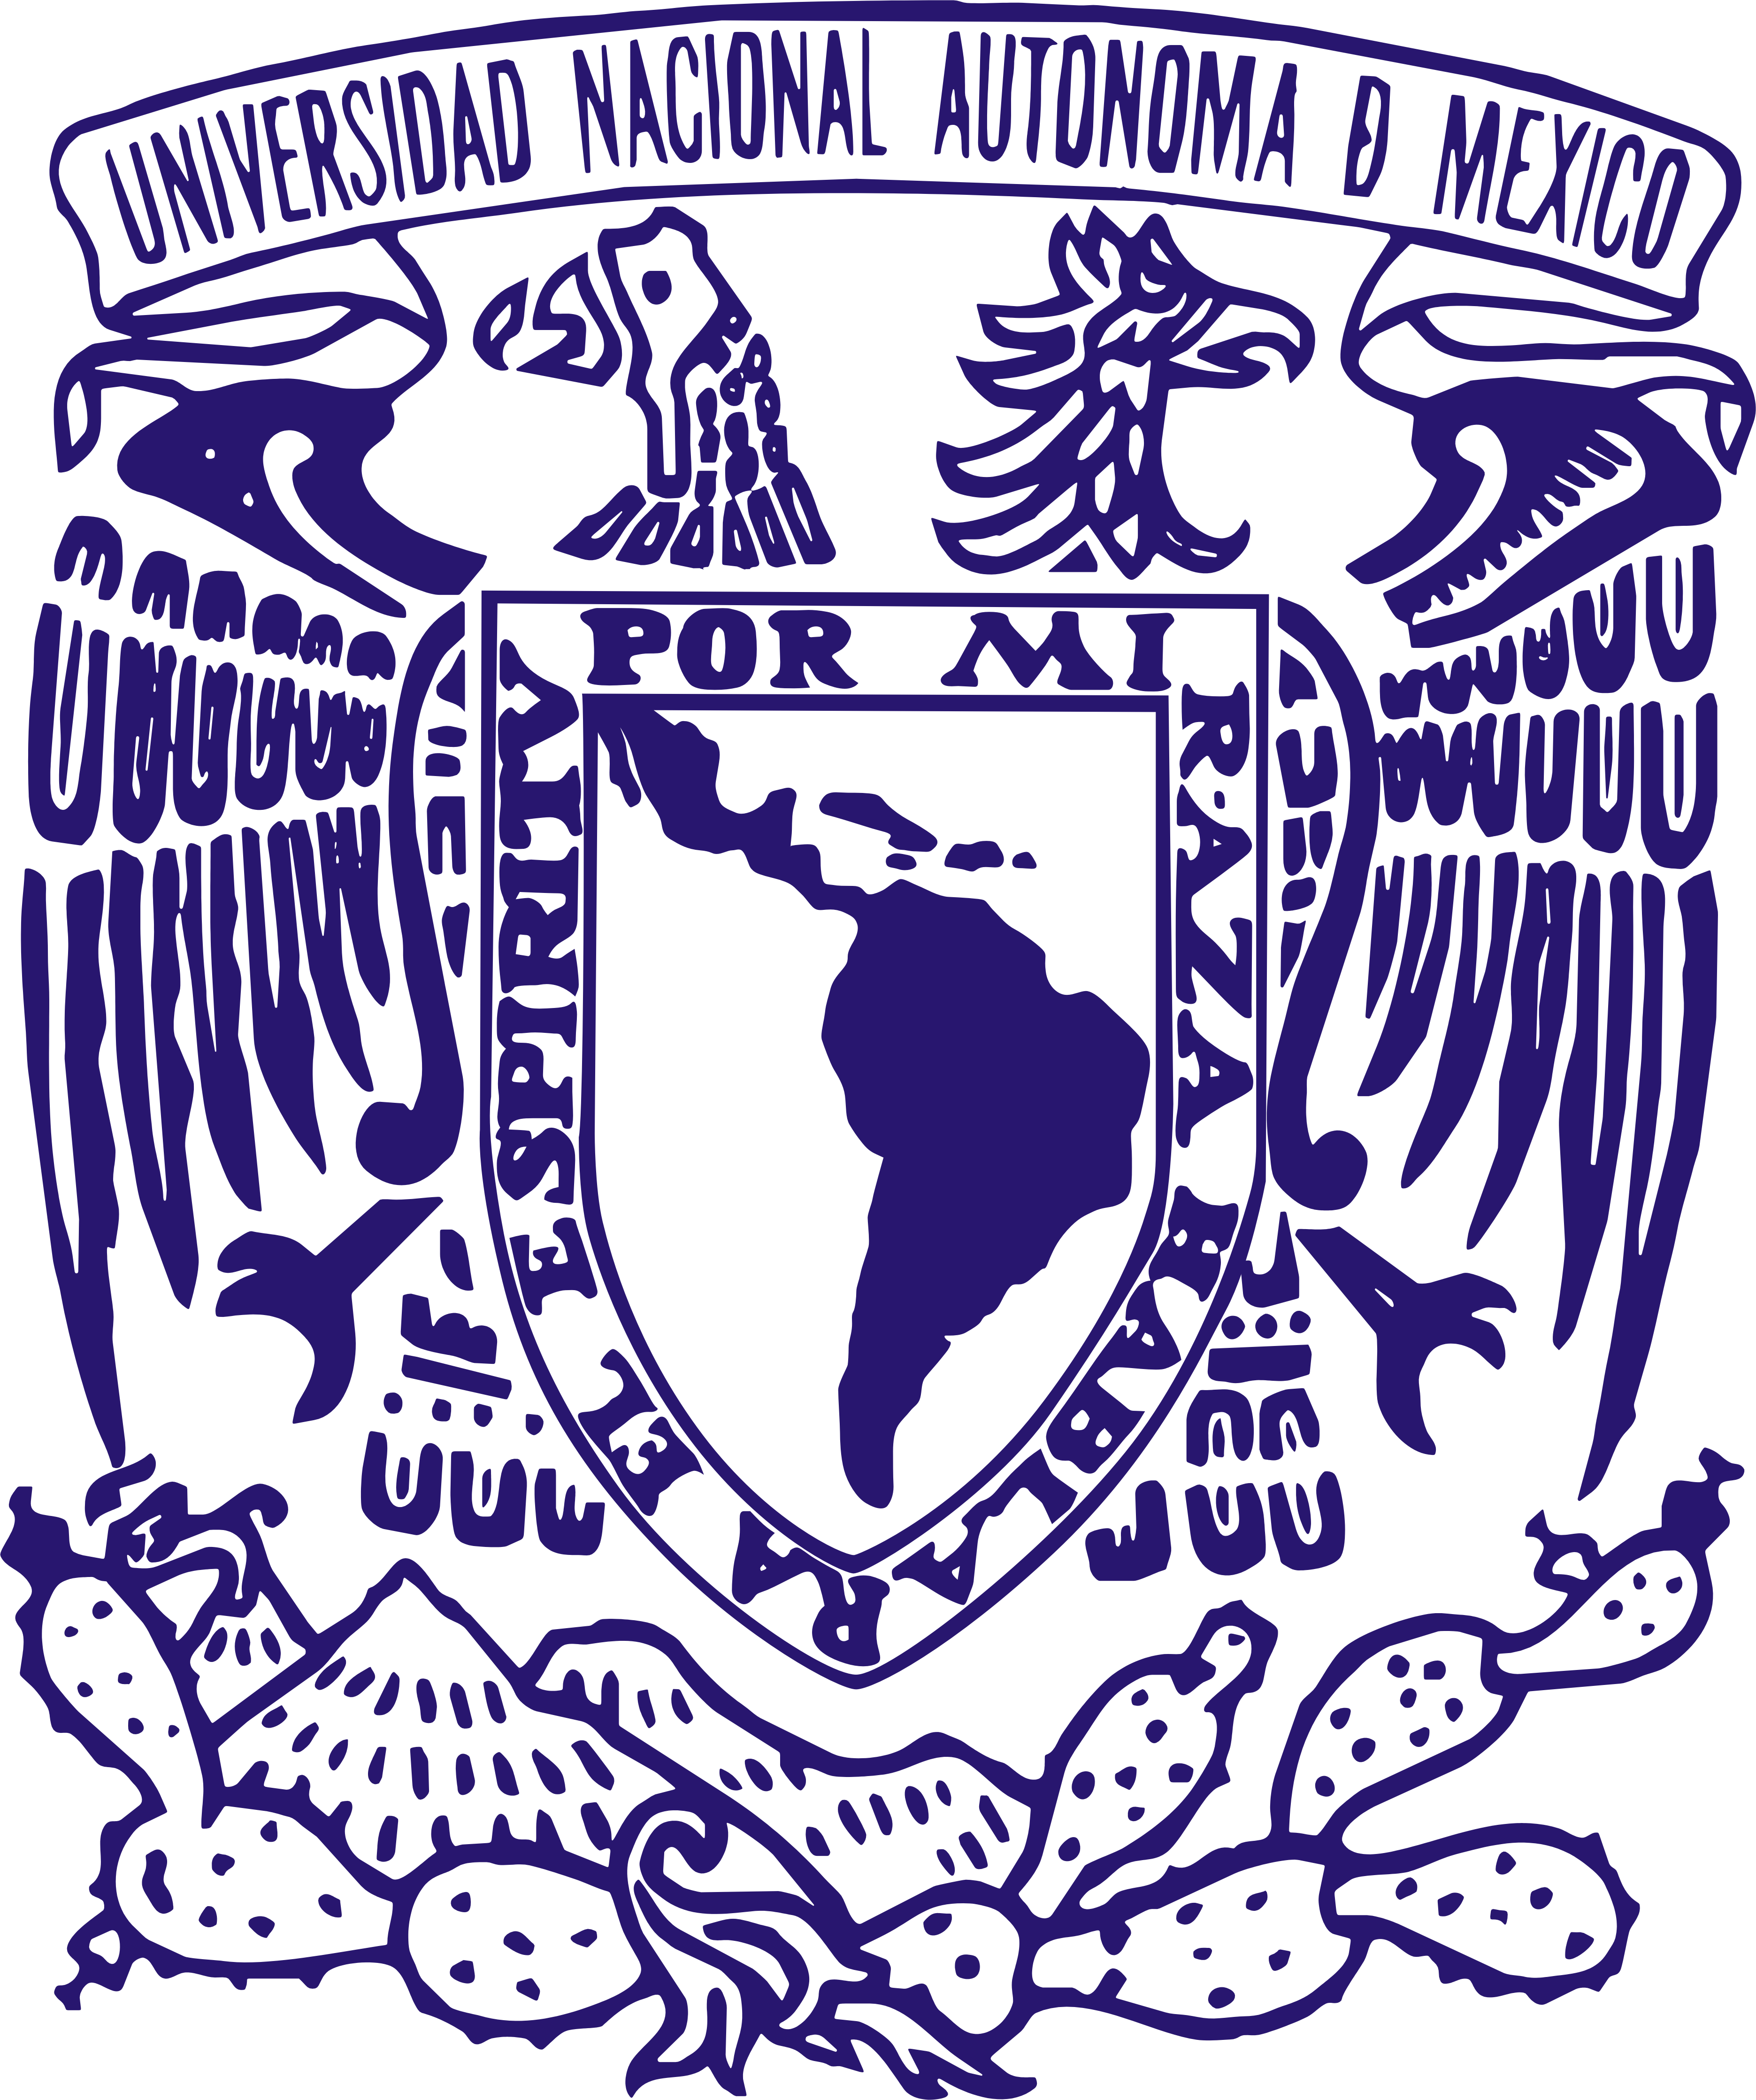
\includegraphics[width=0.18\textwidth]{unam_azul.png}\\
        \textbf{UNIVERSIDAD NACIONAL AUTÓNOMA DE MÉXICO}\\
        MAESTRÍA EN CIENCIAS (NEUROBIOLOGÍA)\\
        INSTITUTO DE NEUROBIOLOGÍA\\
        \vspace{10mm}
        \large
        \textbf{CONECTIVIDAD CEREBRAL EN PACIENTES ADICTOS A COCAÍNA DESPUES DE TRATAMIENTO CON ESTIMULACIÓN MAGNÉTICA TRANSCRANEAL REPETITIVA}\\
        \vspace{10mm}
        \large
        TESIS\\
        \normalsize
        QUE PARA OPTAR POR EL GRADO DE:\\
        MAESTRA EN CIENCIAS\\
        \vspace{10mm}
        PRESENTA:\\
        \large
        \textbf{SOFÍA FERNÁNDEZ LOZANO}\\
        \vfill
        \normalsize
        TUTOR PRINCIPAL\\
        EDUARDO ADRIÁN GARZA VILLARREAL\\
        INSTITUTO NACIONAL DE PSIQUIATRÍA RAMÓN DE LA FUENTE MUÑIZ\\
        \vspace{3mm}
        MIEMBROS DEL COMITÉ TUTOR\\
        SARAEL ALCAUTER SOLORZANO\\
        INB, UNAM\\
        \vspace{1mm}
        ISRAEL VACA PALOMARES\\
        FP, UNAM\\
        \vspace{5mm}
        MÉXICO, CDMX, 2019
    \end{center}
\end{titlepage}
